\section{Motivating example: The impossibility of direct reverse engineering generated code}
\label{sec:motivation}
Let's consider a collaboration scenario between software architects and programmers in developing an event-driven paradigm-based system \ttt{System}. 
Fig. \ref{fig:illustration} (a) and (b) show the current and evolved USM behaviors of \ttt{System}.
%The latter's behavior is described by using a USM as in Fig. \ref{fig:IllustrationExample1}.
%This USM is artificial, and is extracted and customized from the origin in \cite{shuang_formalizing}.
This USM consists of some simple, composite, and pseudo states such as \ttt{choice}, \ttt{connection point expoint}, and \ttt{junction}.

\begin{figure}
	\centering
	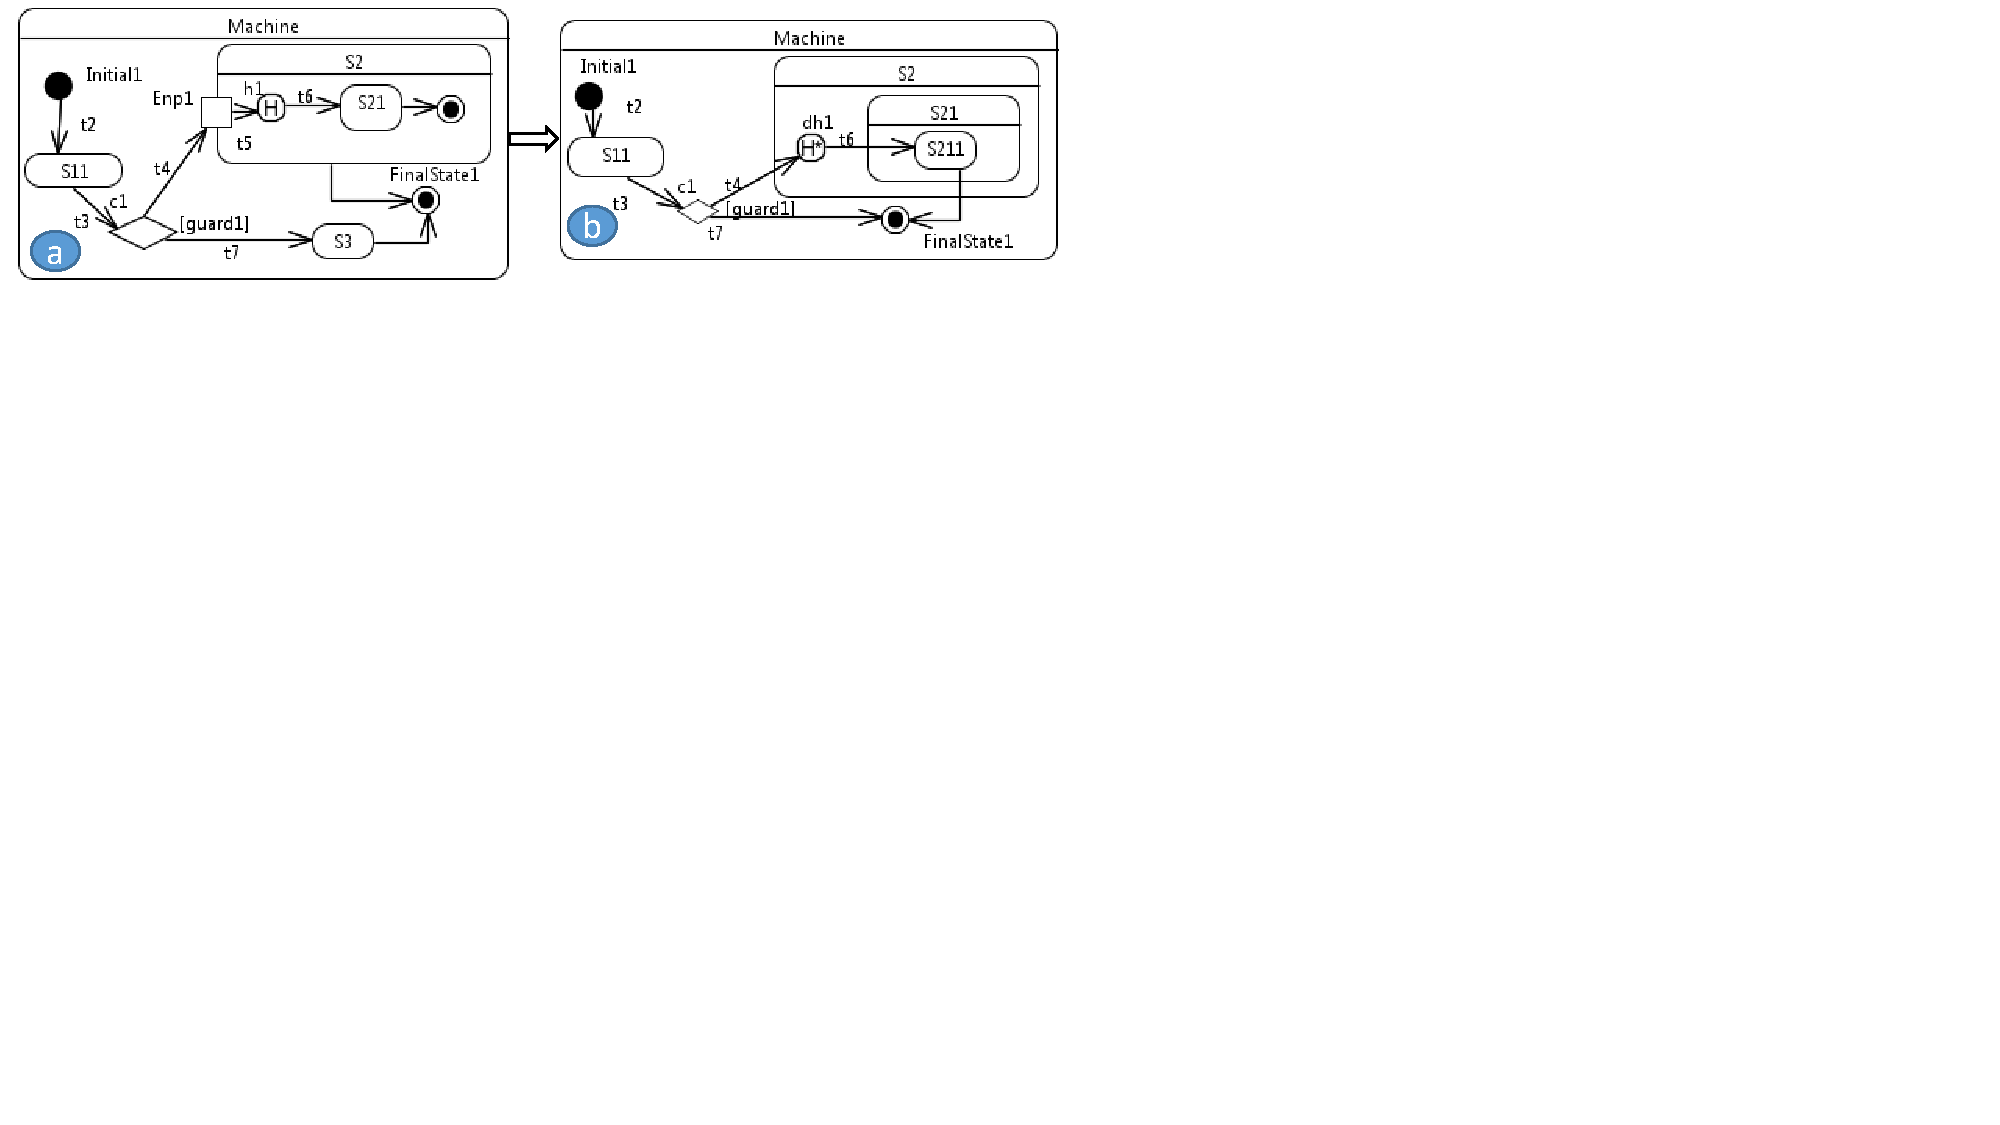
\includegraphics[clip, trim=0cm 10.6cm 18.3cm 0.1cm, width=1.0\columnwidth]{figures/illustration}
	\caption{A USM example (a) and its evolved version (b).} 
	\label{fig:illustration}
\end{figure}


\begin{comment}
\begin{figure}
	\centering
	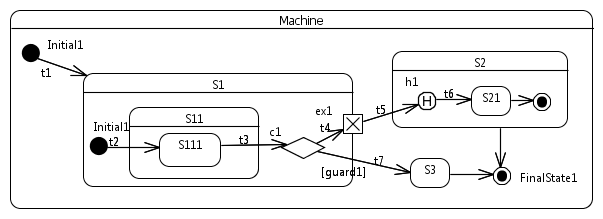
\includegraphics[clip, trim=0.2cm 0.2cm 0.2cm 0.2cm, width=1.0\columnwidth]{figures/IllustrationExample1.png}
	\caption{A USM example} 
	\label{fig:IllustrationExample1}
\end{figure}

\begin{figure}
	\centering
	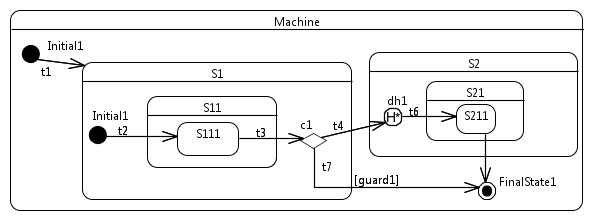
\includegraphics[clip, trim=0.2cm 0.2cm 0.1cm 0.2cm, width=1.0\columnwidth]{figures/IllustrationExample2.png}
	\caption{The evolved version of the USM shown in Fig. \ref{fig:IllustrationExample1}} 
	\label{fig:IllustrationExample2}
\end{figure}
\end{comment}


\begin{figure}
	\centering
	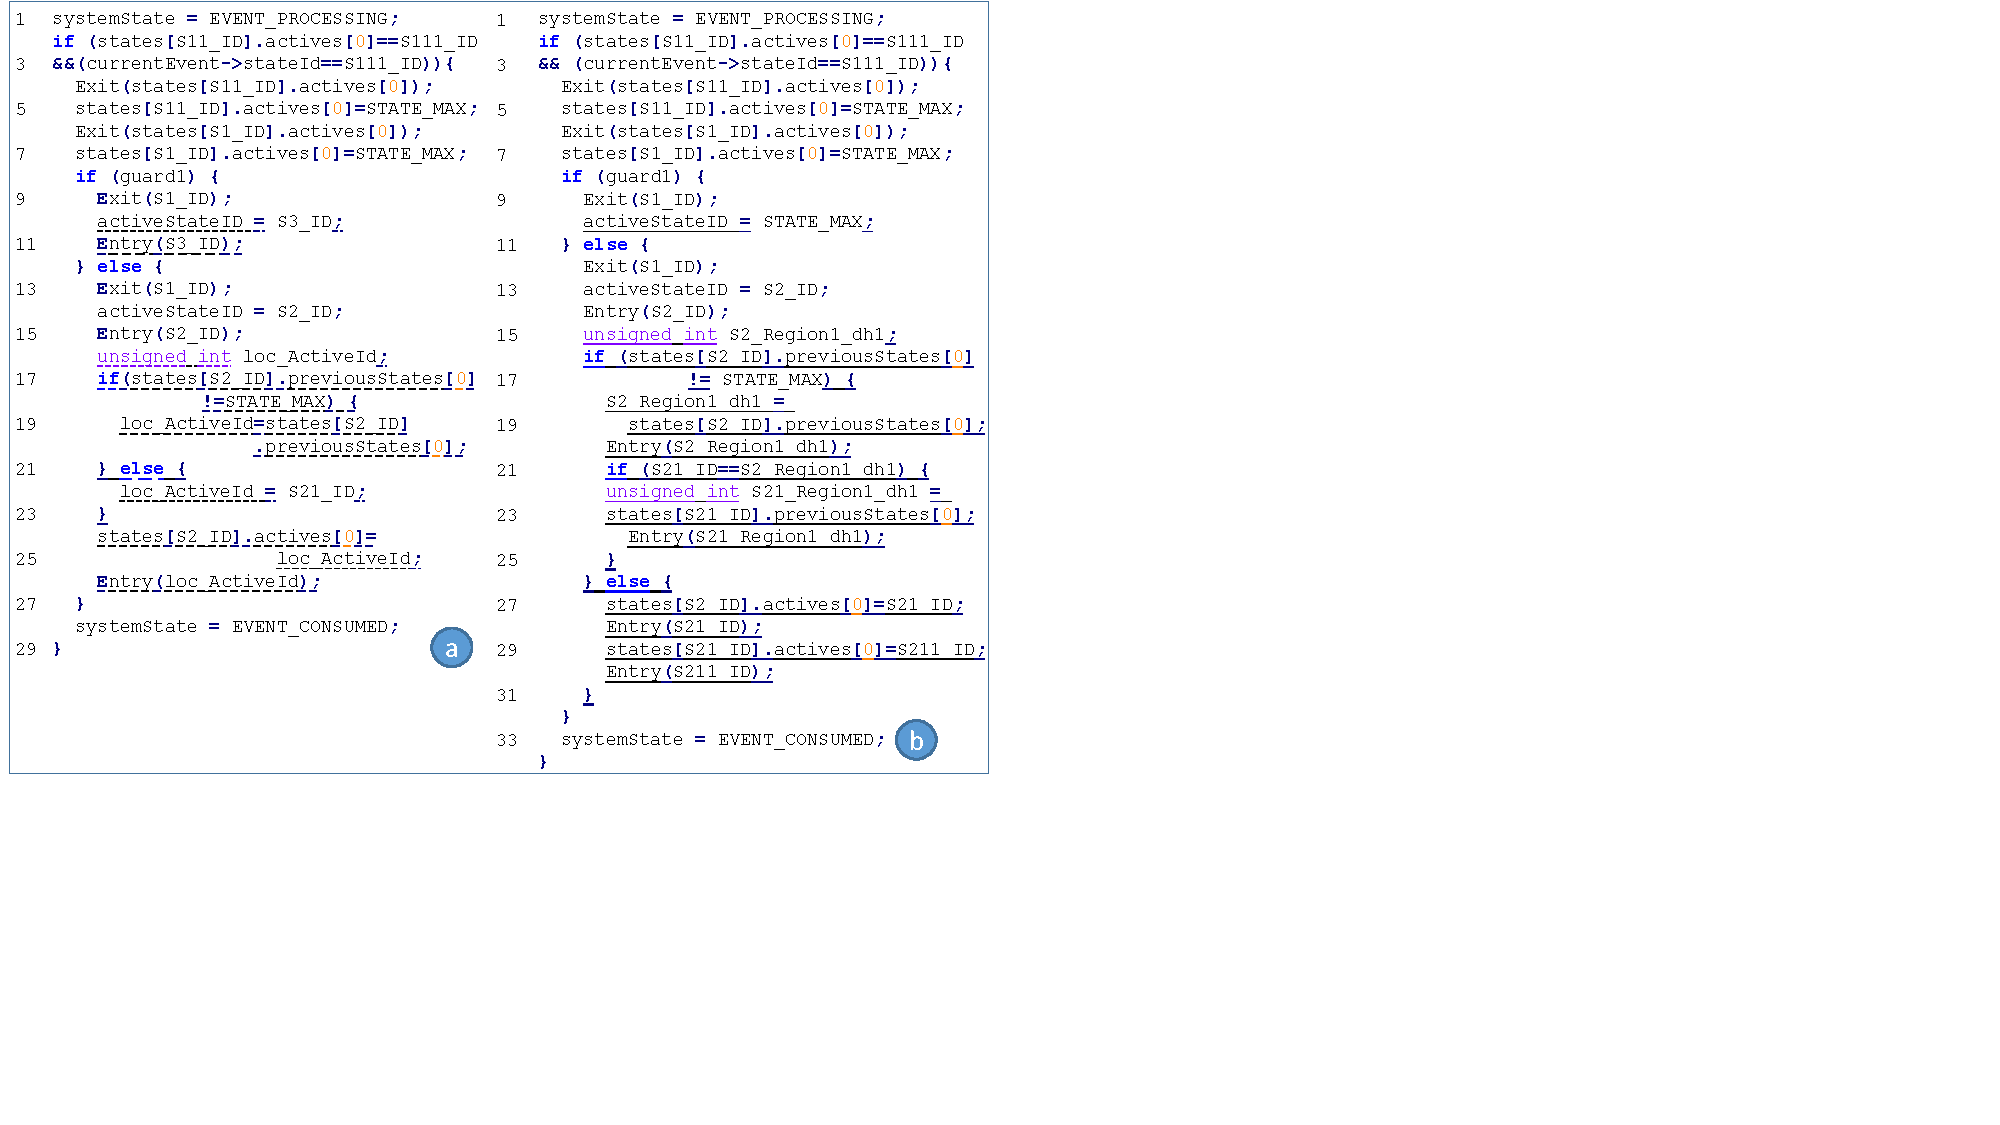
\includegraphics[clip, trim=0.15cm 5.9cm 17.1cm 0.0cm, width=1.04\columnwidth]{figures/highlight.pdf}
	\caption{Codes generated from the state machine example in Fig. \ref{fig:illustration} by using our tool (a) and Rhapsody (b), and their respective evolved versions. The \protect\dashuline{dashed underlined code} segment should evolve to the \protect\uline{simple underlined code}.} 
	\label{fig:generatedcode}
\end{figure}




\begin{comment}
\begin{figure*}
	\centering
	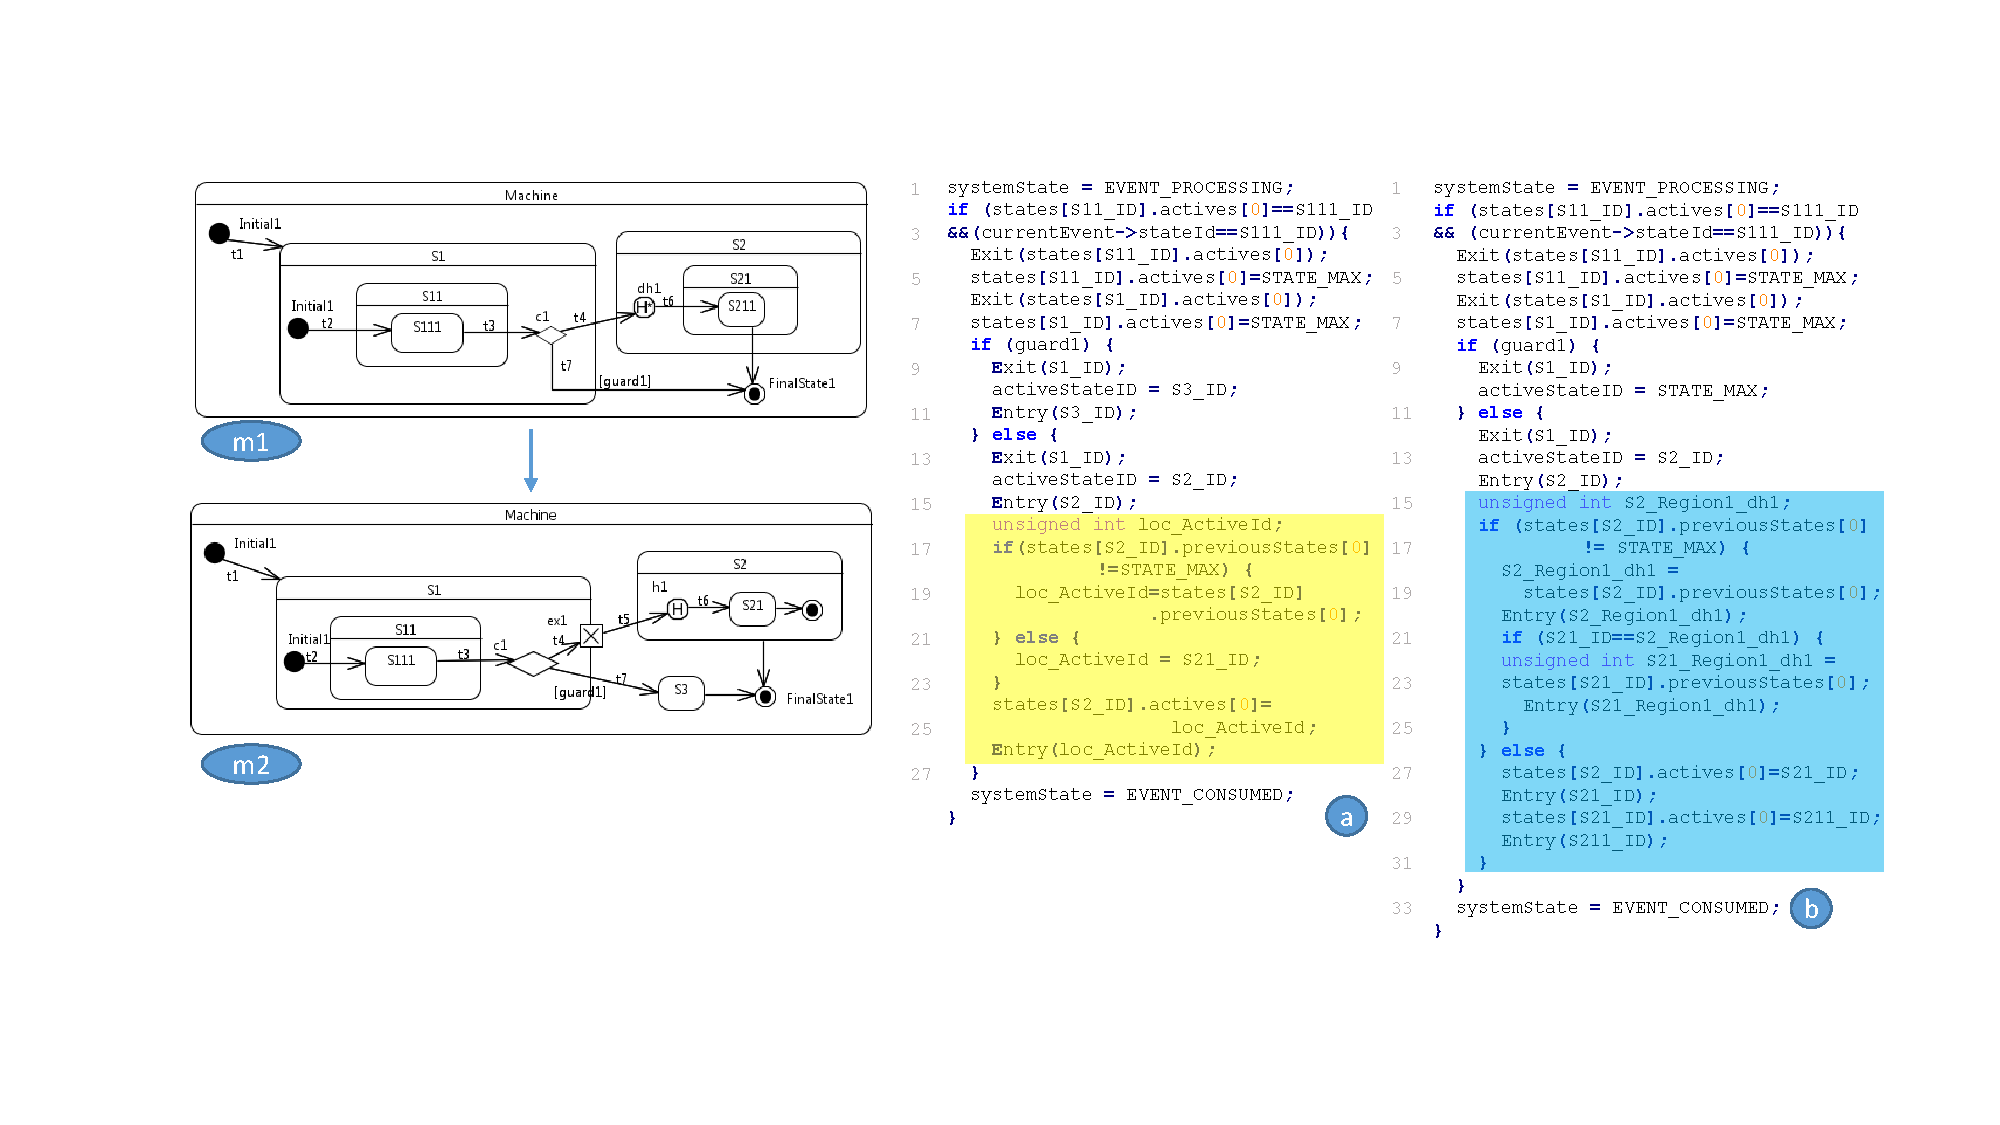
\includegraphics[clip, trim=3.2cm 3.2cm 2.0cm 2.2cm, width=1.0\textwidth]{figures/generatedcodebig2}
	\caption{The evolved version of the USM shown in Fig. \ref{fig:generatedcode}} 
	\label{fig:generatedcode}
\end{figure*}
\end{comment}

%Although many tools have the ability to generate code from USMs, 
A few tools such as IBM Rhapsody \cite{ibm_rhapsody} and ours are able to deal with this example because generating code for pseudo states such as \ttt{expoint} and \ttt{history} is not as simple as states.
Fig. \ref{fig:generatedcode} (a) and (b) show the code segments generated for the transition outgoing from the state \ttt{S111} of the example and its evolved version by using our tool, respectively.

%In this scenario, we assume that, on one hand, programmers prefer to
%use the more familiar textual programming language. 
%On the other hand, software architects, working at higher levels
%of abstraction, tend to favor the use of models, and therefore
%prefer graphical languages for describing the high-level logic behavior by using modeling tools.

%In this scenario, we assume that, for some reasons, the USM should be evolved to the next version as in Fig. \ref{fig:IllustrationExample2}.


For simplification, we assume that no effects are associated with the transitions in the examples.
In Fig. \ref{fig:generatedcode} (a), the code segment checks whether the state \ttt{S111} is active (lines 2-3).
If so, the exit actions of \ttt{S111} and \ttt{S11} are executed sequentially (lines 4 and 6).
The sub-states of \ttt{S11} and \ttt{S1} also become inactive by setting the appropriate values to \ttt{STATE\_MAX} (lines 5 and 7).
The segment then evaluates \ttt{guard1} (lines 8 and 12) to dynamically select which transition outgoing from the choice \ttt{c1} should be taken into account.
The exit action of \ttt{S1} (line 13), the entry action (line 15) and the restoration of the previous active sub-state of \ttt{S2} (lines 16-26) are called if \ttt{guard1} is false. 
Otherwise, \ttt{S1} and \ttt{S3} are exited and entered (lines 9-11), respectively.
The code in Fig. \ref{fig:generatedcode} (b) differs from that of Fig. \ref{fig:generatedcode} (a) by the way the history of \ttt{S2} is restored.
Fig. \ref{fig:generatedcode} (b) executes a deep restoration in lines 14-32 if \ttt{guard1} is evaluated as false.

%It is worth noting that, 
The code generation patterns are not explicitly understandable for the programmers to capture the control flow of the USM. %associated with the code.
Hence, it is challenging to modify the topology of the USM at the code level. 
Even, if the programmers could understand and modify the code %following the used patterns, which require a very high discipline
, it is still very difficult for RTE tools to decipher and reflect the code changes to the model.
Furthermore, 
%code generation patterns produce different code looks.
%As a result, 
it is very hard, if not impossible, to find common rules to reconstruct the original state machine from the code. 
This is the reason why existing RTE tools such as Rhapshody 
%supporting round-trip engineering 
have no way to recover the modified code to the original USM.

Consequently, to interfere the high-level logic behavior of the systems, the programmers must use the click-and-select mechanism of modeling tools, which are, as previously, not encouraged for the programmers to be efficient. 
Furthermore, it does not guarantee the seamless collaboration between the favored practices of the programmers and software architects.  

In the next section, we show how RAOES can handle this collaboration problem.